\begin{enumerate}[label=\thesubsection.\arabic*,ref=\thesubsection.\theenumi]
		\item Find $\abs{\overrightarrow{a}\times\overrightarrow{b}},\text{ if }\overrightarrow{a}=\hat{i}-7\hat{j}+7\hat{k}\text{ and } \overrightarrow{b}=3\hat{i}-2\hat{j}+2\hat{k}$.
	\\
		\solution
		See 
\figref{fig:chapters/10/7/3/4/Fig1}
\begin{figure}[H]
 \begin{center}
  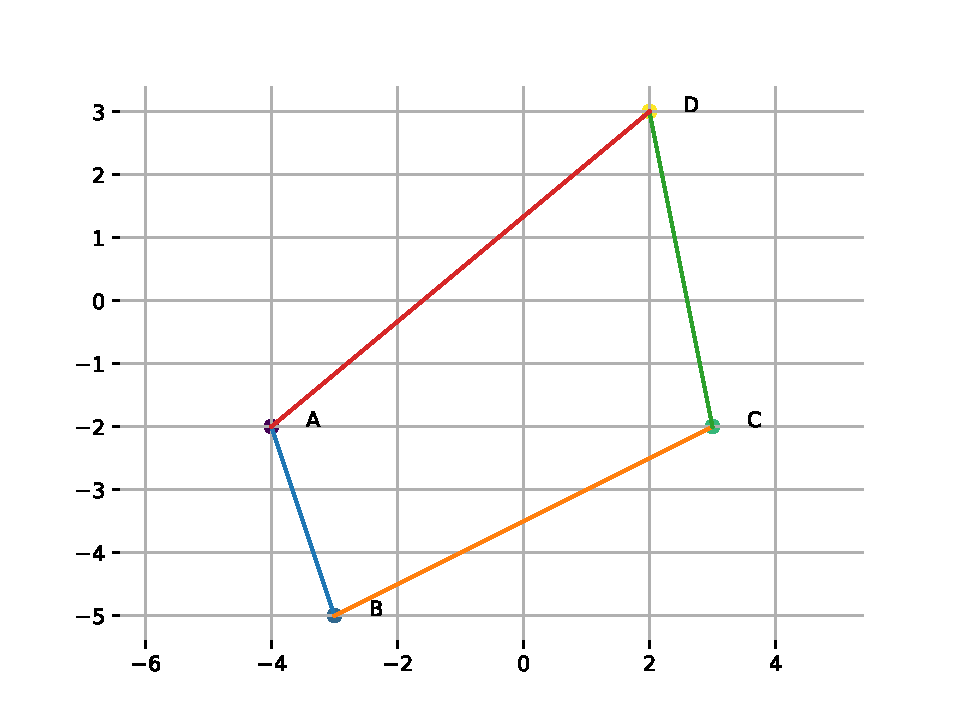
\includegraphics[width=0.75\columnwidth]{chapters/10/7/3/4/figs/fig.pdf}
 \end{center}
\caption{}
\label{fig:chapters/10/7/3/4/Fig1}
\end{figure}
\begin{align}
\because	\vec{A}- \vec{B} =\myvec{-1\\3},\,
	  \vec{A}- \vec{D} =\myvec{-6\\-5},
	  \\
	\vec{B}- \vec{C} =\myvec{-6\\-5},\,
	  \vec{B}- \vec{D} =\myvec{-3\\-8},
	  \\
	  ar(ABD)=\frac{1}{2} \norm{\brak{\vec{A}-\vec{B}}  \times 
   \brak{\vec{A}- \vec{D}}} 
	=	\frac{23}{2}
	\\
	  ar(BCD)=\frac{1}{2} \norm{\brak{\vec{B}-\vec{C}}  \times 
   \brak{\vec{B}- \vec{D}}} 
	=	\frac{33}{2}
	\\
\implies	ar(ABCD)=  ar(ABD) +  ar(BCD)
	= 28
\end{align}

\item Find $\lambda$ and $\mu$ if $(2\hat{i}+6\hat{j}+27\hat{k})\times(\hat{i}+\lambda \hat{j} + \mu \hat{k})=\overrightarrow{0}$.
	\\
		\solution
		See 
\figref{fig:chapters/10/7/3/4/Fig1}
\begin{figure}[H]
 \begin{center}
  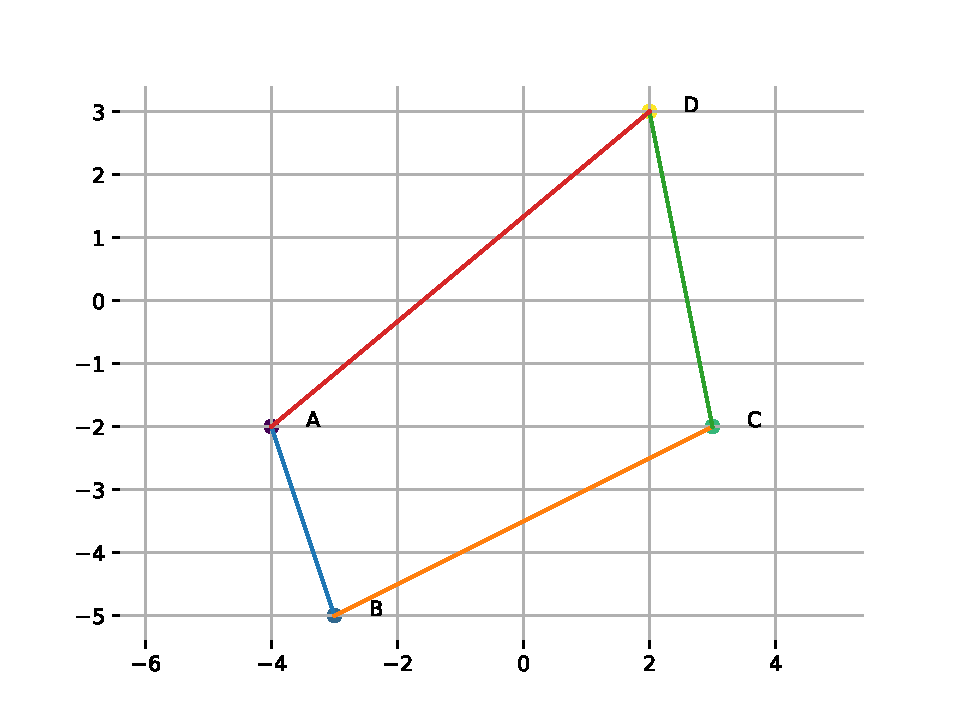
\includegraphics[width=0.75\columnwidth]{chapters/10/7/3/4/figs/fig.pdf}
 \end{center}
\caption{}
\label{fig:chapters/10/7/3/4/Fig1}
\end{figure}
\begin{align}
\because	\vec{A}- \vec{B} =\myvec{-1\\3},\,
	  \vec{A}- \vec{D} =\myvec{-6\\-5},
	  \\
	\vec{B}- \vec{C} =\myvec{-6\\-5},\,
	  \vec{B}- \vec{D} =\myvec{-3\\-8},
	  \\
	  ar(ABD)=\frac{1}{2} \norm{\brak{\vec{A}-\vec{B}}  \times 
   \brak{\vec{A}- \vec{D}}} 
	=	\frac{23}{2}
	\\
	  ar(BCD)=\frac{1}{2} \norm{\brak{\vec{B}-\vec{C}}  \times 
   \brak{\vec{B}- \vec{D}}} 
	=	\frac{33}{2}
	\\
\implies	ar(ABCD)=  ar(ABD) +  ar(BCD)
	= 28
\end{align}

\item Find the area of the triangle with vertices $A(1, 1, 2), B(2, 3, 5)$ and $C(1, 5, 5)$.
	\\
		\solution
		See 
\figref{fig:chapters/10/7/3/4/Fig1}
\begin{figure}[H]
 \begin{center}
  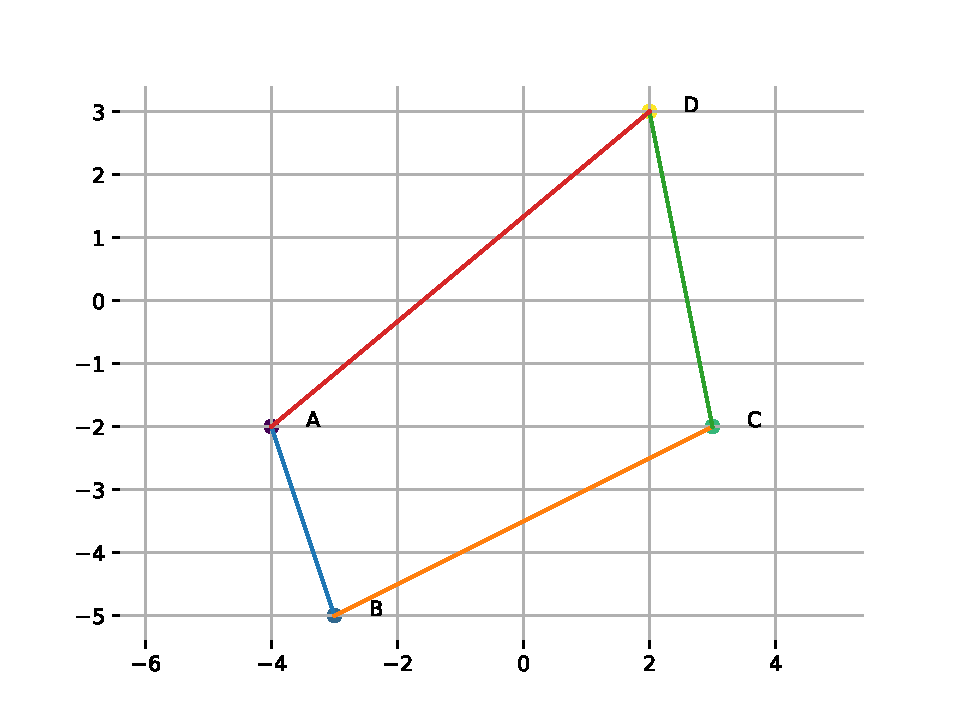
\includegraphics[width=0.75\columnwidth]{chapters/10/7/3/4/figs/fig.pdf}
 \end{center}
\caption{}
\label{fig:chapters/10/7/3/4/Fig1}
\end{figure}
\begin{align}
\because	\vec{A}- \vec{B} =\myvec{-1\\3},\,
	  \vec{A}- \vec{D} =\myvec{-6\\-5},
	  \\
	\vec{B}- \vec{C} =\myvec{-6\\-5},\,
	  \vec{B}- \vec{D} =\myvec{-3\\-8},
	  \\
	  ar(ABD)=\frac{1}{2} \norm{\brak{\vec{A}-\vec{B}}  \times 
   \brak{\vec{A}- \vec{D}}} 
	=	\frac{23}{2}
	\\
	  ar(BCD)=\frac{1}{2} \norm{\brak{\vec{B}-\vec{C}}  \times 
   \brak{\vec{B}- \vec{D}}} 
	=	\frac{33}{2}
	\\
\implies	ar(ABCD)=  ar(ABD) +  ar(BCD)
	= 28
\end{align}

\item Find the area of the parallelogram whose adjacent sides are determined by the vectors $\overrightarrow{a}=\hat{i}-\hat{j}+3\hat{k}$ and $\overrightarrow{b}=2\hat{i}-7\hat{j}+\hat{k}$.
	\\
		\solution
		See 
\figref{fig:chapters/10/7/3/4/Fig1}
\begin{figure}[H]
 \begin{center}
  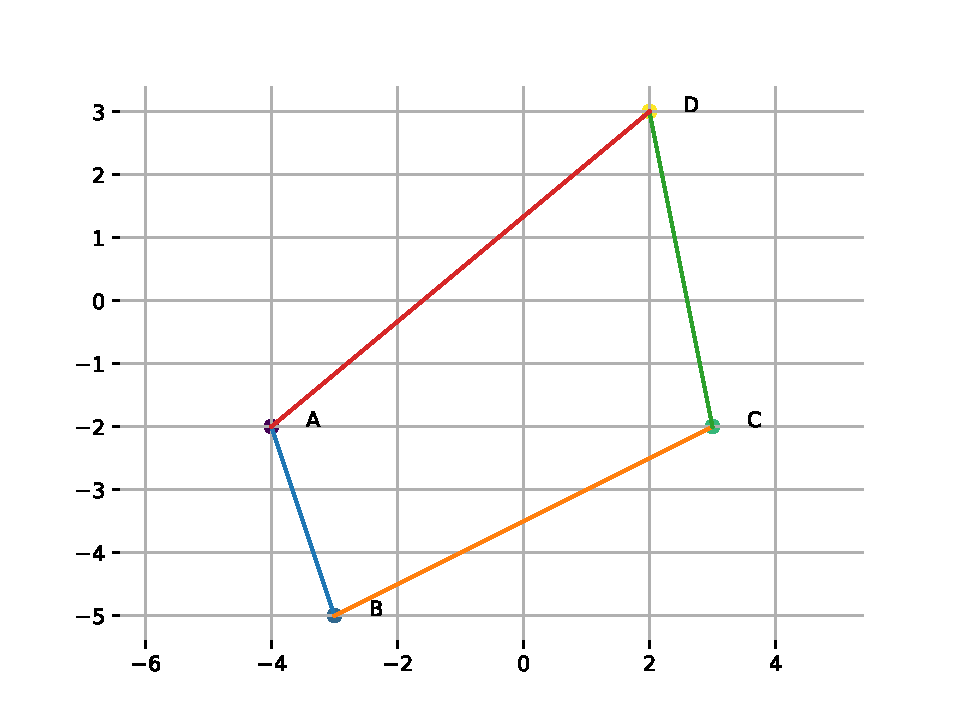
\includegraphics[width=0.75\columnwidth]{chapters/10/7/3/4/figs/fig.pdf}
 \end{center}
\caption{}
\label{fig:chapters/10/7/3/4/Fig1}
\end{figure}
\begin{align}
\because	\vec{A}- \vec{B} =\myvec{-1\\3},\,
	  \vec{A}- \vec{D} =\myvec{-6\\-5},
	  \\
	\vec{B}- \vec{C} =\myvec{-6\\-5},\,
	  \vec{B}- \vec{D} =\myvec{-3\\-8},
	  \\
	  ar(ABD)=\frac{1}{2} \norm{\brak{\vec{A}-\vec{B}}  \times 
   \brak{\vec{A}- \vec{D}}} 
	=	\frac{23}{2}
	\\
	  ar(BCD)=\frac{1}{2} \norm{\brak{\vec{B}-\vec{C}}  \times 
   \brak{\vec{B}- \vec{D}}} 
	=	\frac{33}{2}
	\\
\implies	ar(ABCD)=  ar(ABD) +  ar(BCD)
	= 28
\end{align}

\item Find the area of a rhombus if its vertices are $A(3,0), B(4,5), C(-1,4)$  and  $D(-2,-1)$ taken in order. 
	\\
		\solution
	See 
\figref{fig:chapters/10/7/3/4/Fig1}
\begin{figure}[H]
 \begin{center}
  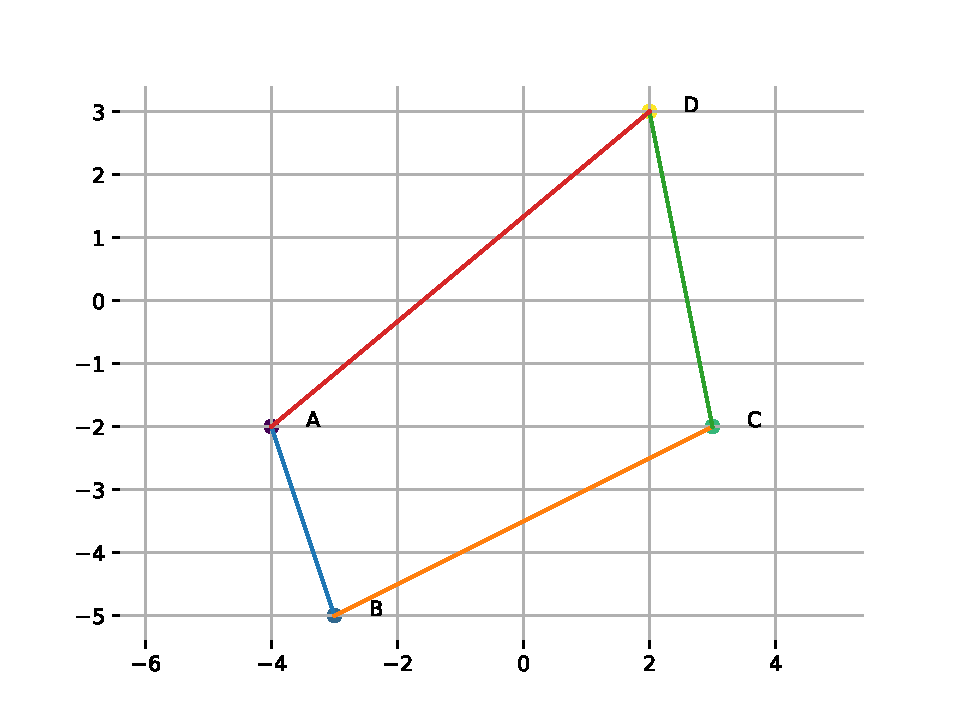
\includegraphics[width=0.75\columnwidth]{chapters/10/7/3/4/figs/fig.pdf}
 \end{center}
\caption{}
\label{fig:chapters/10/7/3/4/Fig1}
\end{figure}
\begin{align}
\because	\vec{A}- \vec{B} =\myvec{-1\\3},\,
	  \vec{A}- \vec{D} =\myvec{-6\\-5},
	  \\
	\vec{B}- \vec{C} =\myvec{-6\\-5},\,
	  \vec{B}- \vec{D} =\myvec{-3\\-8},
	  \\
	  ar(ABD)=\frac{1}{2} \norm{\brak{\vec{A}-\vec{B}}  \times 
   \brak{\vec{A}- \vec{D}}} 
	=	\frac{23}{2}
	\\
	  ar(BCD)=\frac{1}{2} \norm{\brak{\vec{B}-\vec{C}}  \times 
   \brak{\vec{B}- \vec{D}}} 
	=	\frac{33}{2}
	\\
\implies	ar(ABCD)=  ar(ABD) +  ar(BCD)
	= 28
\end{align}

\item Let the vectors $\overrightarrow{a}$ and $\overrightarrow{b}$ be such that $|\overrightarrow{a}| = 3$ and $|\overrightarrow{b}| = \dfrac{\sqrt{2}}{3}$, then $\overrightarrow{a} \times \overrightarrow{b}$ is a unit vector, if the angle between $\overrightarrow{a}$ and $\overrightarrow{b}$ is
	\begin{multicols}{2}
	\begin{enumerate}
\item $\frac{\pi}{6}$
\item $\frac{\pi}{4}$
\item $\frac{\pi}{3}$
\item $\frac{\pi}{2}$
\end{enumerate}
	\end{multicols}
		\solution
		See 
\figref{fig:chapters/10/7/3/4/Fig1}
\begin{figure}[H]
 \begin{center}
  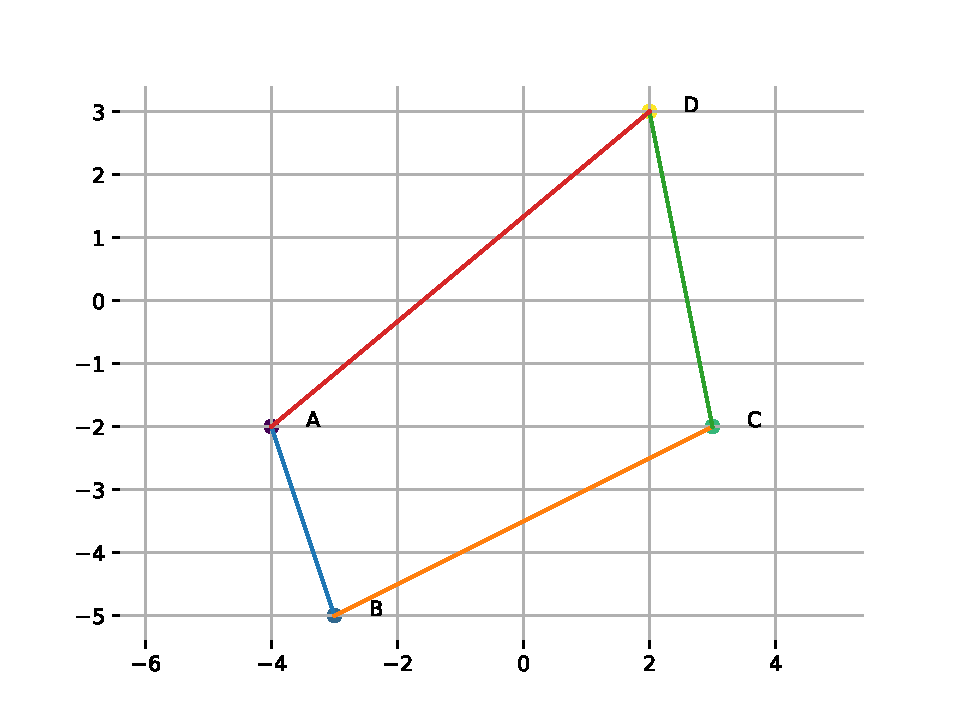
\includegraphics[width=0.75\columnwidth]{chapters/10/7/3/4/figs/fig.pdf}
 \end{center}
\caption{}
\label{fig:chapters/10/7/3/4/Fig1}
\end{figure}
\begin{align}
\because	\vec{A}- \vec{B} =\myvec{-1\\3},\,
	  \vec{A}- \vec{D} =\myvec{-6\\-5},
	  \\
	\vec{B}- \vec{C} =\myvec{-6\\-5},\,
	  \vec{B}- \vec{D} =\myvec{-3\\-8},
	  \\
	  ar(ABD)=\frac{1}{2} \norm{\brak{\vec{A}-\vec{B}}  \times 
   \brak{\vec{A}- \vec{D}}} 
	=	\frac{23}{2}
	\\
	  ar(BCD)=\frac{1}{2} \norm{\brak{\vec{B}-\vec{C}}  \times 
   \brak{\vec{B}- \vec{D}}} 
	=	\frac{33}{2}
	\\
\implies	ar(ABCD)=  ar(ABD) +  ar(BCD)
	= 28
\end{align}

\item Area of a rectangle having vertices A, B, C and D with position vectors $ -\hat{i}+ \frac{1}{2} \hat{j}+4\hat{k}, \hat{i}+ \frac{1}{2} \hat{j}+4\hat{k}, \hat{i}-\frac{1}{2} \hat{j}+4\hat{k}$ and $-\hat{i}- \frac{1}{2} \hat{j}+4\hat{k}$, respectively is
	\\
		\solution
		See 
\figref{fig:chapters/10/7/3/4/Fig1}
\begin{figure}[H]
 \begin{center}
  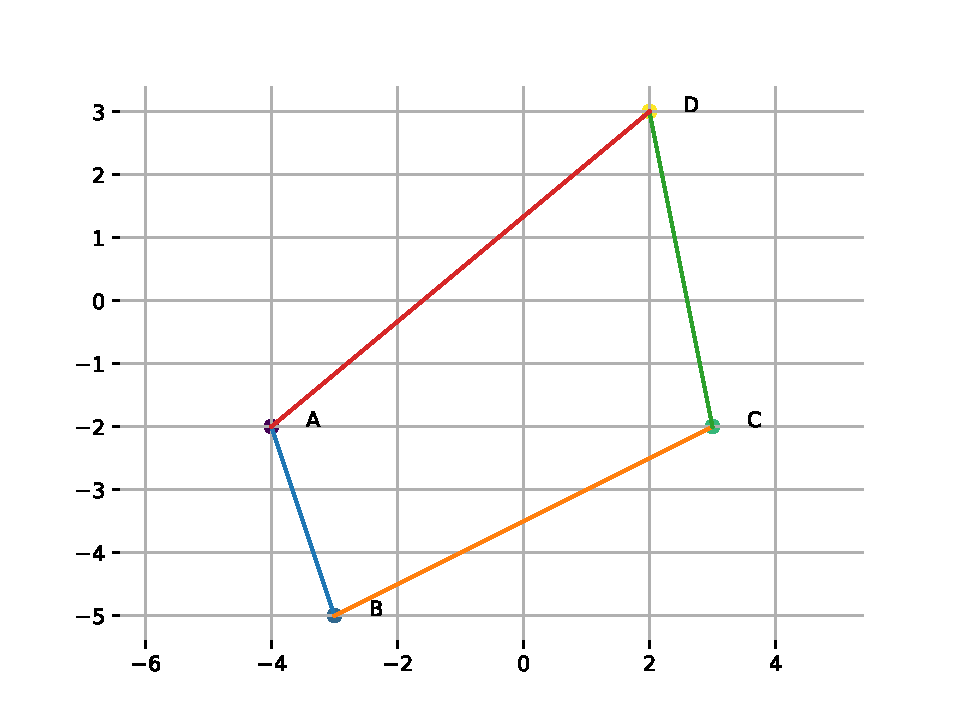
\includegraphics[width=0.75\columnwidth]{chapters/10/7/3/4/figs/fig.pdf}
 \end{center}
\caption{}
\label{fig:chapters/10/7/3/4/Fig1}
\end{figure}
\begin{align}
\because	\vec{A}- \vec{B} =\myvec{-1\\3},\,
	  \vec{A}- \vec{D} =\myvec{-6\\-5},
	  \\
	\vec{B}- \vec{C} =\myvec{-6\\-5},\,
	  \vec{B}- \vec{D} =\myvec{-3\\-8},
	  \\
	  ar(ABD)=\frac{1}{2} \norm{\brak{\vec{A}-\vec{B}}  \times 
   \brak{\vec{A}- \vec{D}}} 
	=	\frac{23}{2}
	\\
	  ar(BCD)=\frac{1}{2} \norm{\brak{\vec{B}-\vec{C}}  \times 
   \brak{\vec{B}- \vec{D}}} 
	=	\frac{33}{2}
	\\
\implies	ar(ABCD)=  ar(ABD) +  ar(BCD)
	= 28
\end{align}

\item Find the area of the triangle whose vertices are 
\begin{enumerate}
\item $(2, 3), (–1, 0), (2, – 4)$
\item $(–5, –1), (3, –5), (5, 2)$ 
\end{enumerate}
		\label{10/7/3/1}
\solution
		\begin{align}
\vec{D}=\frac{\vec{B}+\vec{C}}{2}
=\myvec{4\\ 0},
\\
	\vec{A}- \vec{B} =\myvec{1\\ -4},\,
	  \vec{A}- \vec{D} =\myvec{0\\ -6}
	  \\
	  \implies
  ar(ABD)=\frac{1}{2} \norm{\brak{\vec{A}-\vec{B}}  \times 
   \brak{\vec{A}- \vec{D}}} 
	       =3	
	       \\
	\vec{A}- \vec{C} =\myvec{-1\\ -8},\,
	  \vec{A}- \vec{D} =\myvec{0\\ -6}
	  \\
	  \implies
  ar(ACD)=\frac{1}{2} \norm{\brak{\vec{A}-\vec{C}}  \times 
   \brak{\vec{A}- \vec{D}}} 
   \\
	= 3 =
ar(ABD)
\end{align}
See  
\figref{fig:10/7/3/5/}.
\begin{figure}[H]
\centering
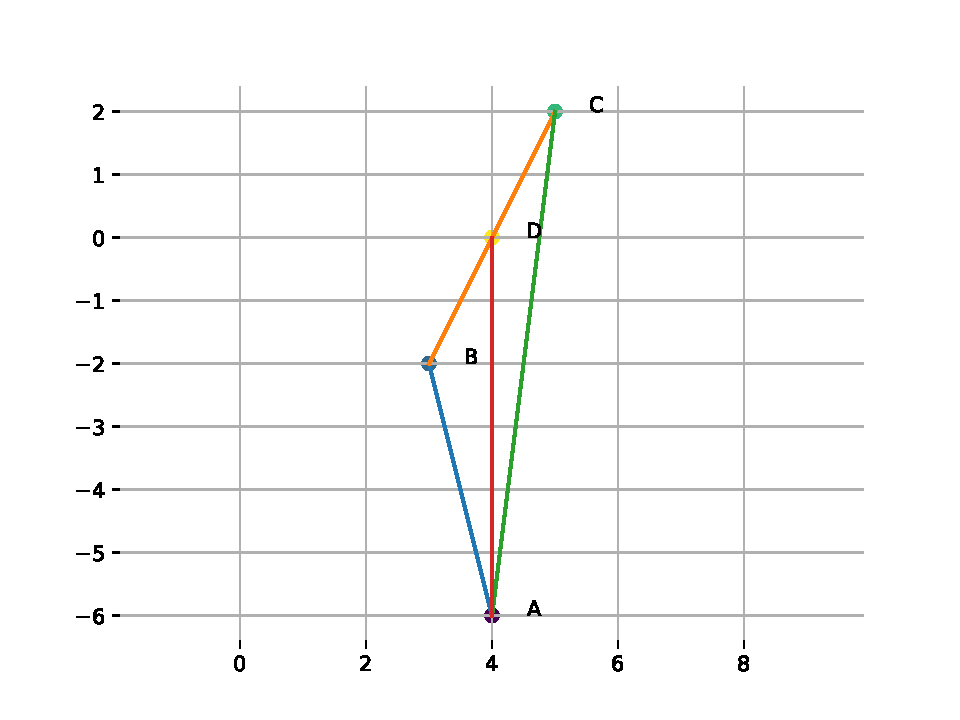
\includegraphics[width=0.75\columnwidth]{chapters/10/7/3/5/figs/fig.pdf}
\caption{}
\label{fig:10/7/3/5/}
\end{figure} 

\item Find the area of the triangle formed by joining the mid-points of the sides of the triangle whose vertices are $A(0, –1), B(2, 1)$  and  $C(0, 3)$. Find the ratio of this area to the area of the given triangle.
	\\
\solution
		See 
\figref{fig:chapters/10/7/3/4/Fig1}
\begin{figure}[H]
 \begin{center}
  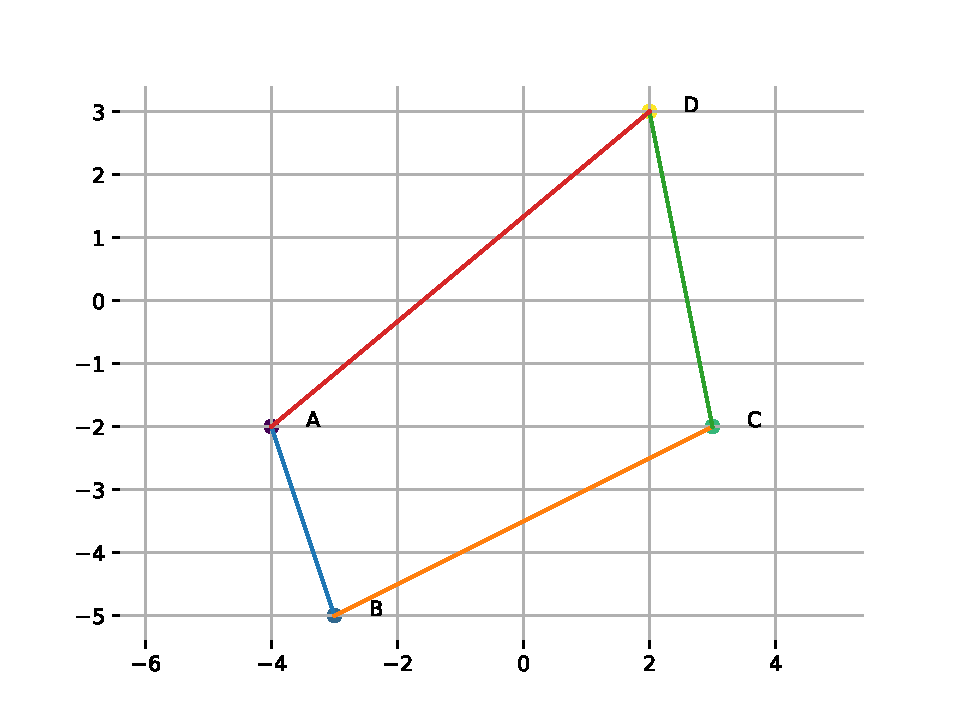
\includegraphics[width=0.75\columnwidth]{chapters/10/7/3/4/figs/fig.pdf}
 \end{center}
\caption{}
\label{fig:chapters/10/7/3/4/Fig1}
\end{figure}
\begin{align}
\because	\vec{A}- \vec{B} =\myvec{-1\\3},\,
	  \vec{A}- \vec{D} =\myvec{-6\\-5},
	  \\
	\vec{B}- \vec{C} =\myvec{-6\\-5},\,
	  \vec{B}- \vec{D} =\myvec{-3\\-8},
	  \\
	  ar(ABD)=\frac{1}{2} \norm{\brak{\vec{A}-\vec{B}}  \times 
   \brak{\vec{A}- \vec{D}}} 
	=	\frac{23}{2}
	\\
	  ar(BCD)=\frac{1}{2} \norm{\brak{\vec{B}-\vec{C}}  \times 
   \brak{\vec{B}- \vec{D}}} 
	=	\frac{33}{2}
	\\
\implies	ar(ABCD)=  ar(ABD) +  ar(BCD)
	= 28
\end{align}


\item Find the area of the quadrilateral whose vertices, taken in order, are $A(– 4, – 2), B(– 3, – 5), C(3, – 2)$  and $ D(2, 3)$.
	\\
\solution
		See 
\figref{fig:chapters/10/7/3/4/Fig1}
\begin{figure}[H]
 \begin{center}
  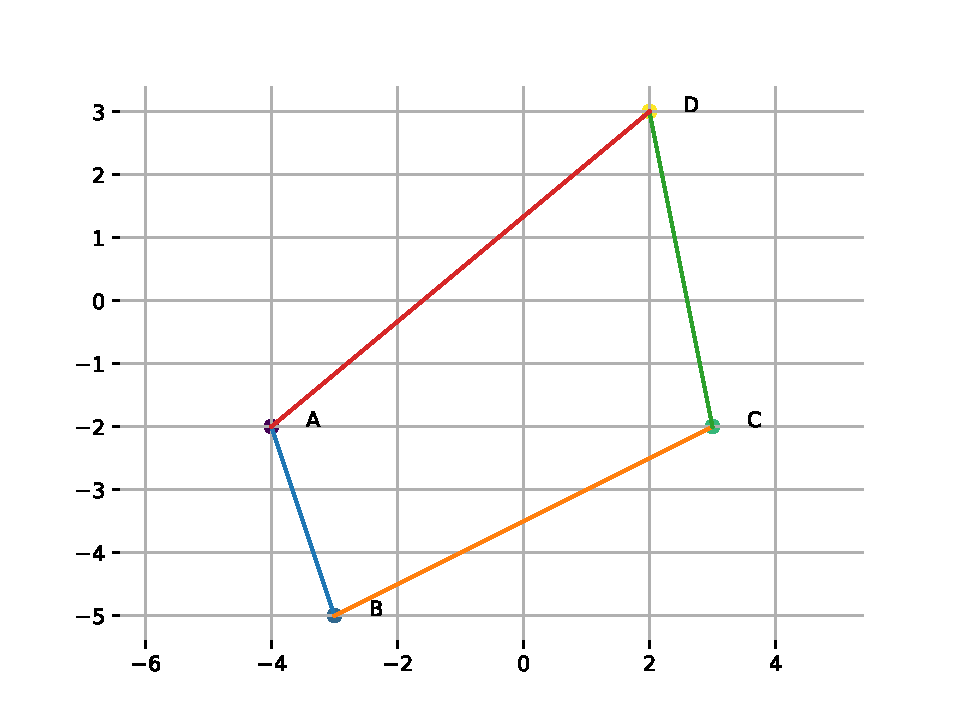
\includegraphics[width=0.75\columnwidth]{chapters/10/7/3/4/figs/fig.pdf}
 \end{center}
\caption{}
\label{fig:chapters/10/7/3/4/Fig1}
\end{figure}
\begin{align}
\because	\vec{A}- \vec{B} =\myvec{-1\\3},\,
	  \vec{A}- \vec{D} =\myvec{-6\\-5},
	  \\
	\vec{B}- \vec{C} =\myvec{-6\\-5},\,
	  \vec{B}- \vec{D} =\myvec{-3\\-8},
	  \\
	  ar(ABD)=\frac{1}{2} \norm{\brak{\vec{A}-\vec{B}}  \times 
   \brak{\vec{A}- \vec{D}}} 
	=	\frac{23}{2}
	\\
	  ar(BCD)=\frac{1}{2} \norm{\brak{\vec{B}-\vec{C}}  \times 
   \brak{\vec{B}- \vec{D}}} 
	=	\frac{33}{2}
	\\
\implies	ar(ABCD)=  ar(ABD) +  ar(BCD)
	= 28
\end{align}


\item Verify that a median of a triangle divides it into two triangles of equal areas for $\triangle ABC$ whose vertices are $\vec{A}(4, -6), \vec{B}(3, 2), \text{ and } \vec{C}(5, 2)$. 
		\label{10/7/3/5}
		\\
\solution
		\begin{align}
\vec{D}=\frac{\vec{B}+\vec{C}}{2}
=\myvec{4\\ 0},
\\
	\vec{A}- \vec{B} =\myvec{1\\ -4},\,
	  \vec{A}- \vec{D} =\myvec{0\\ -6}
	  \\
	  \implies
  ar(ABD)=\frac{1}{2} \norm{\brak{\vec{A}-\vec{B}}  \times 
   \brak{\vec{A}- \vec{D}}} 
	       =3	
	       \\
	\vec{A}- \vec{C} =\myvec{-1\\ -8},\,
	  \vec{A}- \vec{D} =\myvec{0\\ -6}
	  \\
	  \implies
  ar(ACD)=\frac{1}{2} \norm{\brak{\vec{A}-\vec{C}}  \times 
   \brak{\vec{A}- \vec{D}}} 
   \\
	= 3 =
ar(ABD)
\end{align}
See  
\figref{fig:10/7/3/5/}.
\begin{figure}[H]
\centering
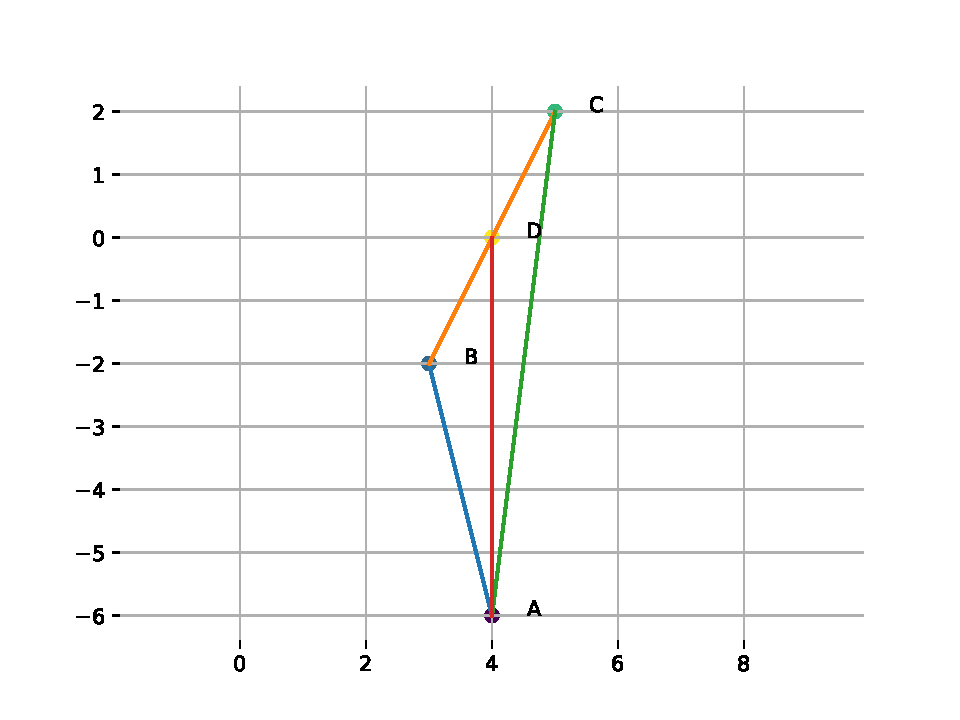
\includegraphics[width=0.75\columnwidth]{chapters/10/7/3/5/figs/fig.pdf}
\caption{}
\label{fig:10/7/3/5/}
\end{figure} 

\item The two adjacent sides of a parallelogram are 
$\vec{a}= 2\hat{i}-4\hat{j}+5\hat{k}$  and  $\vec{b} =\hat{i}-2\hat{j}-3\hat{k}$.
Find the unit vector parallel to its diagonal. Also, find its area.\\
	\solution
		See 
\figref{fig:chapters/10/7/3/4/Fig1}
\begin{figure}[H]
 \begin{center}
  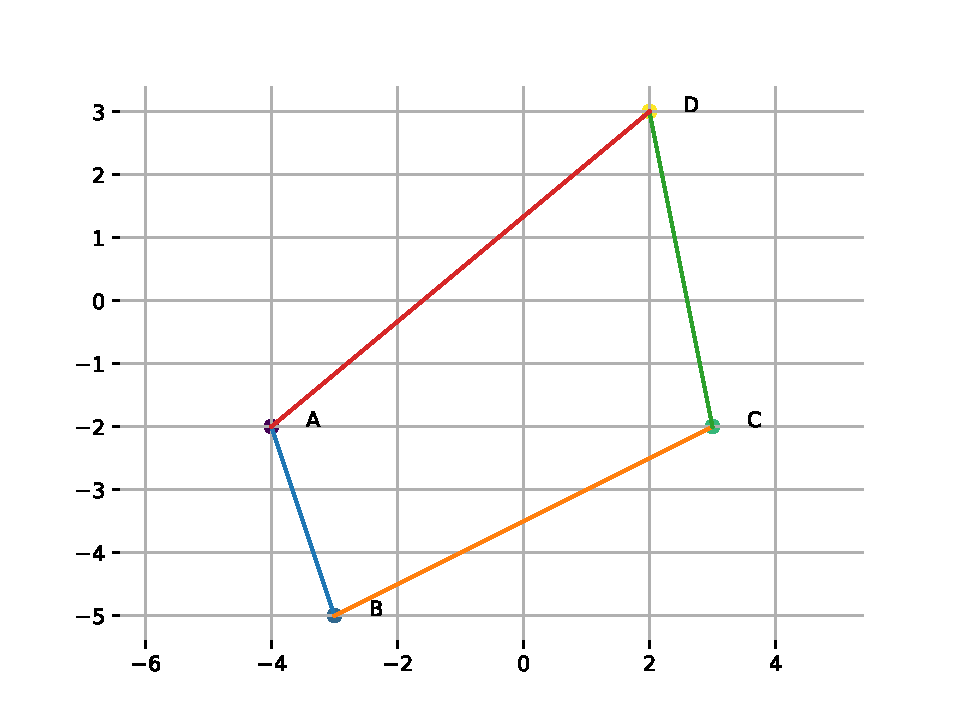
\includegraphics[width=0.75\columnwidth]{chapters/10/7/3/4/figs/fig.pdf}
 \end{center}
\caption{}
\label{fig:chapters/10/7/3/4/Fig1}
\end{figure}
\begin{align}
\because	\vec{A}- \vec{B} =\myvec{-1\\3},\,
	  \vec{A}- \vec{D} =\myvec{-6\\-5},
	  \\
	\vec{B}- \vec{C} =\myvec{-6\\-5},\,
	  \vec{B}- \vec{D} =\myvec{-3\\-8},
	  \\
	  ar(ABD)=\frac{1}{2} \norm{\brak{\vec{A}-\vec{B}}  \times 
   \brak{\vec{A}- \vec{D}}} 
	=	\frac{23}{2}
	\\
	  ar(BCD)=\frac{1}{2} \norm{\brak{\vec{B}-\vec{C}}  \times 
   \brak{\vec{B}- \vec{D}}} 
	=	\frac{33}{2}
	\\
\implies	ar(ABCD)=  ar(ABD) +  ar(BCD)
	= 28
\end{align}

\item The vertices of a $\triangle ABC$ are $\vec{A}(4,6), \vec{B}(1,5)$ and  $\vec{C}(7,2)$. A line is drawn to intersect sides $AB$ and $AC$ at $\vec{D}$ and $\vec{E}$ respectively, such that $\frac{AD}{AB} = \frac{AE}{AC} = \frac{1}{4}$. Calculate the area of $\triangle ADE$ and compare it with the area of the $\triangle ABC$.
\\
\solution
	The desired vector is
\begin{align}
\frac{1}{2}\myvec{2\\3\\4} +  \frac{1}{2}\myvec{4\\1\\-2} =\myvec{3\\2\\1} 
\end{align}




    \item Draw a quadrilateral in the Cartesian plane, whose vertices are 
    \begin{align}
        \vec{A} = \myvec{-4\\5},\, \vec{B} = \myvec{0\\7},\, 
        \vec{C} = \myvec{5\\-5},\, \vec{D} = \myvec{-4\\-2}.
    \end{align}
    Also, find its area.
\label{chapters/11/10/1/1}
   \\ 
    \solution 
See 
\figref{fig:chapters/10/7/3/4/Fig1}
\begin{figure}[H]
 \begin{center}
  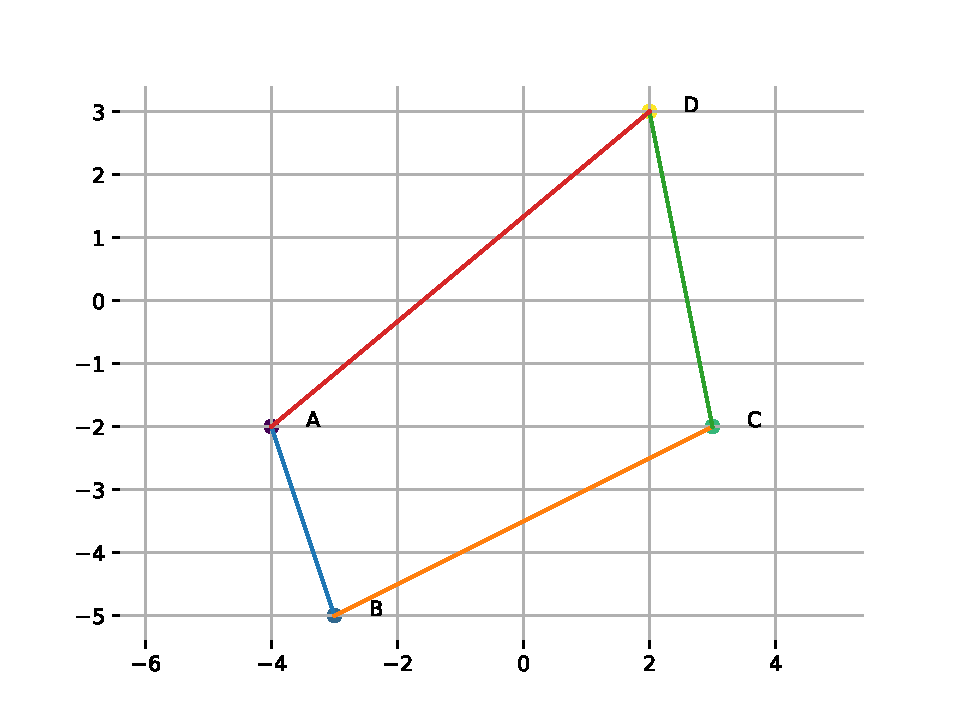
\includegraphics[width=0.75\columnwidth]{chapters/10/7/3/4/figs/fig.pdf}
 \end{center}
\caption{}
\label{fig:chapters/10/7/3/4/Fig1}
\end{figure}
\begin{align}
\because	\vec{A}- \vec{B} =\myvec{-1\\3},\,
	  \vec{A}- \vec{D} =\myvec{-6\\-5},
	  \\
	\vec{B}- \vec{C} =\myvec{-6\\-5},\,
	  \vec{B}- \vec{D} =\myvec{-3\\-8},
	  \\
	  ar(ABD)=\frac{1}{2} \norm{\brak{\vec{A}-\vec{B}}  \times 
   \brak{\vec{A}- \vec{D}}} 
	=	\frac{23}{2}
	\\
	  ar(BCD)=\frac{1}{2} \norm{\brak{\vec{B}-\vec{C}}  \times 
   \brak{\vec{B}- \vec{D}}} 
	=	\frac{33}{2}
	\\
\implies	ar(ABCD)=  ar(ABD) +  ar(BCD)
	= 28
\end{align}

\item Find the area of region bounded by the triangle whose
	vertices are $(1, 0), (2, 2)$ and $(3, 1)$. 
\item Find the area of region bounded by the triangle whose vertices
	are $(– 1, 0), (1, 3)$  and  $(3, 2)$. 
\item Find the area of the $\triangle ABC$, coordinates of whose vertices are $\vec{A}(2, 0), \vec{B}(4, 5)$ and $\vec{C}(6, 3)$.
\item The area of a triangle with vertices $\vec{A}(3, 0), \vec{B}(7, 0)$ and  $\vec{C}(8, 4)$ is
\begin{enumerate}
\item 14
\item 28
\item 8
\item 6
\end{enumerate}
\item Find the area of the triangle whose vertices are $(-8,4),(-6,6)$ and $(-3,9)$.
\item If $\vec{D}\brak{\frac{-1}{2},\frac{5}{2}},\vec{E}(7,3)$ and $\vec{F}\brak{\frac{7}{2},\frac{7}{2}}$ are the midpoints of sides of $\triangle ABC$, find the area of the $\triangle ABC$.
\item Find the sine of the angle between the vectors $\vec{a}=3\hat{i}+\hat{j}+2\hat{k}$ $\text{ and }$ $\vec{b}=2\hat{i}-2\hat{j}+4\hat{k}$.
\item Using vectors, find the area of $\triangle{ABC}$ with vertices A(1,2,3), B(2,-1,4) and C(4,5,-1).
\item Find the area of the parallelogram whose diagonals are $2\hat{i}-\hat{j}+\hat{k}$ and $\hat{i}+3\hat{j}-\hat{k}$.

\item The vector from origin to the points A and B are $\vec{a}$ = $2\hat{i}-3\hat{j}+2\hat{k}$ and  $\vec{b}$ = $2\hat{i}+3\hat{j}+\hat{k}$, respectively, then the area of $\triangle {OAB}$ is
	\begin{enumerate}
\item 340 
\item $\sqrt{25}$
\item $\sqrt{229}$
\item $\frac{1}{2}\sqrt{229}$
\end{enumerate}
\item If $\vec{a} = \hat{i}+\hat{j}+\hat{k}$ and $\vec{b} = \hat{j}-\hat{k}$, find a vector $\vec{c}$ such that $\vec{a}\times\vec{c} = \vec{b}$ and $\vec{a}\cdot \vec{c}$ = 3.
%
\item The area of the quadrilateral ABCD, where A$(0,4,1)$, B$(2,3,-1)$, C$(4,5,0)$ and D$(2,6,2)$, is equal to 
\begin{enumerate}
	\item 9 sq. units
	\item 18 sq. units 
	\item 27 sq. units 
	\item 81 sq. units
\end{enumerate}
\item Find the area of region bounded by the triangle whose vertices are $(-1, 1), (0, 5)$ and $(3, 2)$.
\item The value of $\hat{i}\cdot(\hat{j}\times\hat{k})+\hat{j}\cdot(\hat{i}\times\hat{k})+\hat{k}\cdot(\hat{i}\times\hat{j})$ is
\begin{enumerate}
\item 0
\item -1
\item 1
\item 3
\end{enumerate}
\item The value of $\hat{i}\cdot (\hat{j}\times\hat{k})+\hat{j}\cdot (\hat{i}\times\hat{k})+\hat{k}\cdot (\hat{i}\times\hat{j})$ is
\begin{enumerate}
\item 0
\item -1
\item 1
\item 3
\end{enumerate}
\item Find area of the triangle with vertices at the point given in each of the following:
\begin{enumerate}
\item $(1,0), (6,0), (4,3)$
\item $(2.7), (1,1), (10,8)$
\item $(-2,-3), (3,2), (-1,8)$
\end{enumerate}
\item If area of triangle is 35 square units with vertices $(2,6), (5,-4)$ and $(k,4)$. Then $k$ is:
\begin{enumerate}
\item $12$
\item $-2$
\item $-12,-2$
\item $12, -2$
\end{enumerate}
\item Find values of $k$ if area of triangle is 4 square units and vertices are
\begin{enumerate}
\item $(k,0), (4,0), (0,2)$
\item $(-2,0), (0,4), (0,k)$
\end{enumerate}
\item Find the area of the triangle whose vertices are $(1,-1), (-4,6)$ and $(-3,5)$.
\item Find the area of a triangle formed by the points $A(5,2), B(4,7)$ and $(7,-4)$.
\item Find the area of the triangle formed by the points $P(-1.5,3), Q(6,-2)$ and $R(-3,4)$.
\item If $A(-5,7), B(-4,-5), C(-1,-6)$ and $D(4,5)$ are the vertices of a quadrilateral, find the area of quadrilateral ABCD.
\item Find the area of the triangle whose vertices are $(3,8), (-4,2)$ and $(5,1)$.
\item Find $\abs{\overrightarrow{a} \times \overrightarrow{b}}$, if $\overrightarrow{a} = 2\hat{i} +\hat{j} +3\hat{k}$, and $\overrightarrow{b} = 3\hat{i} +5\hat{j} -2\hat{k}$.
\item Find the area of a triangle having the points $A(1,1,1), B(1,2,3)$ and $C(2,3,1)$ as its vertices.
\item Find the area of a parallelogram whose adjacent sides are given by the vectors $\overrightarrow{a}=3\hat{i} +\hat{j} +4\hat{k}$ and $\overrightarrow{b}=\hat{i} -\hat{j} +\hat{k}$.
\end{enumerate}

